\documentclass[10pt]{beamer}\usepackage[]{graphicx}\usepackage[]{color}
%% maxwidth is the original width if it is less than linewidth
%% otherwise use linewidth (to make sure the graphics do not exceed the margin)
\makeatletter
\def\maxwidth{ %
  \ifdim\Gin@nat@width>\linewidth
    \linewidth
  \else
    \Gin@nat@width
  \fi
}
\makeatother

\definecolor{fgcolor}{rgb}{0.345, 0.345, 0.345}
\newcommand{\hlnum}[1]{\textcolor[rgb]{0.686,0.059,0.569}{#1}}%
\newcommand{\hlstr}[1]{\textcolor[rgb]{0.192,0.494,0.8}{#1}}%
\newcommand{\hlcom}[1]{\textcolor[rgb]{0.678,0.584,0.686}{\textit{#1}}}%
\newcommand{\hlopt}[1]{\textcolor[rgb]{0,0,0}{#1}}%
\newcommand{\hlstd}[1]{\textcolor[rgb]{0.345,0.345,0.345}{#1}}%
\newcommand{\hlkwa}[1]{\textcolor[rgb]{0.161,0.373,0.58}{\textbf{#1}}}%
\newcommand{\hlkwb}[1]{\textcolor[rgb]{0.69,0.353,0.396}{#1}}%
\newcommand{\hlkwc}[1]{\textcolor[rgb]{0.333,0.667,0.333}{#1}}%
\newcommand{\hlkwd}[1]{\textcolor[rgb]{0.737,0.353,0.396}{\textbf{#1}}}%
\let\hlipl\hlkwb

\usepackage{framed}
\makeatletter
\newenvironment{kframe}{%
 \def\at@end@of@kframe{}%
 \ifinner\ifhmode%
  \def\at@end@of@kframe{\end{minipage}}%
  \begin{minipage}{\columnwidth}%
 \fi\fi%
 \def\FrameCommand##1{\hskip\@totalleftmargin \hskip-\fboxsep
 \colorbox{shadecolor}{##1}\hskip-\fboxsep
     % There is no \\@totalrightmargin, so:
     \hskip-\linewidth \hskip-\@totalleftmargin \hskip\columnwidth}%
 \MakeFramed {\advance\hsize-\width
   \@totalleftmargin\z@ \linewidth\hsize
   \@setminipage}}%
 {\par\unskip\endMakeFramed%
 \at@end@of@kframe}
\makeatother

\definecolor{shadecolor}{rgb}{.97, .97, .97}
\definecolor{messagecolor}{rgb}{0, 0, 0}
\definecolor{warningcolor}{rgb}{1, 0, 1}
\definecolor{errorcolor}{rgb}{1, 0, 0}
\newenvironment{knitrout}{}{} % an empty environment to be redefined in TeX

\usepackage{alltt}
\usepackage{amsmath}
\usepackage{amssymb}
\usepackage{geometry}
\usepackage{graphicx}
\usepackage{url}
\usepackage{bm}

\makeatletter
\let \@sverbatim \@verbatim
\def \@verbatim {\@sverbatim \verbatimplus}
{\catcode`'=13 \gdef \verbatimplus{\catcode`'=13 \chardef '=13 }} 
\makeatother

\newcommand{\RSS}{\text{RSS}}
\IfFileExists{upquote.sty}{\usepackage{upquote}}{}
\begin{document}

% --------------------------------------------
\begin{frame}
\large
Lecture 15:\\ 
Box-Cox Transformations\\
STAT 632, Spring 2020\\
\end{frame}

% --------------------------------------------
\begin{frame}{Transforming the Response}
The Box-Cox method is a popular way to estimate a transformation for the response variable.\\
\vspace{10pt}

For a strictly positive response variable $Y$, the Box-Cox family of transformations is given by:
\begin{align*}
h(Y, \lambda) =
\begin{cases}
\frac{Y^{\lambda} - 1}{\lambda},& \text{if $\lambda \neq 0$}\\
\log(Y),& \text{if $\lambda = 0$}
\end{cases}
\end{align*}
Transformations, previously discussed, such as the square root ($\lambda = 1/2$) and the logarithm ($\lambda = 0$) are members of the Box-Cox family.  Note that the $\log()$ function is assumed to be base $e$ (also denoted as $\ln()$, the natural logarithm). 
\end{frame}

%--------------------------------------------
\begin{frame}
Properties of Box-Cox transformations:
\begin{itemize}
\item $h(Y, \lambda)$ is a continuous function of $\lambda$
\item The logarithmic transformation is a member of this family, since
$$\lim_{\lambda \rightarrow 0} \frac{Y^{\lambda} - 1}{\lambda} = \log(Y)$$
\item Dividing by $\lambda$ preserves the direction of $Y$, which would otherwise be reversed when $\lambda$ is negative.  As an illustration
\begin{table}
\begin{tabular}{llll}
\hline
$Y$ & $Y^{-1}$ & $\frac{Y^{-1}}{-1}$ & $\frac{Y^{-1}-1}{-1}$\\
\hline
1 & 1 & -1 & 0\\
2 & 1/2 & -1/2 & 1/2\\
3 & 1/3 & -1/3 & 2/3\\
4 & 1/4 & -1/4 & 3/4
\end{tabular}
\end{table}
\end{itemize}
\end{frame}

%--------------------------------------------
\begin{frame}
The parameter $\lambda$ is estimated by maximizing the log-likelihood function\footnote{See Sheather, pp. 228--230, for some background on maximum likelihood estimation in the context of multiple linear regression.}:
\begin{align*}
l(\lambda) = -\frac{n}{2} \log(\RSS(\lambda) / n) + (\lambda - 1) \sum_{i=1}^n \log y_i
\end{align*}
where $\RSS(\lambda)$ is the residuals sum of squares when $h(y_i, \lambda)$ is the response.  More specifically,
\begin{align*}
\RSS(\lambda) = \sum_{i=1}^n [h(y_i, \lambda) - \hat{\beta}_0 - \hat{\beta}_1 x_{i1} - \cdots - \hat{\beta}_p x_{ip}]^2
\end{align*}
where $\hat{\beta}_0, \cdots, \hat{\beta}_p$ are the least squares estimates of the parameters for transformed regression model $h(Y_i, \lambda)  = \beta_0 + \beta_1 x_{i1} + \cdots + \beta_p x_{ip} + e$.\\
\vspace{10pt}

%Note that $l(\lambda)$ is often called the \emph{profile log-likelihood}, since we maximize $l(\lambda)$ with respect to $\lambda$, while fixing the other parameters, $\beta_0, \cdots, \beta_p, \sigma^2$, at their maximum likelihood estimates, $\hat{\beta}_0, \cdots, \hat{\beta}_p, \hat{\sigma}^2$.
\end{frame}

%--------------------------------------------
\begin{frame}{Example: Modeling Defective Rates (Sheather, Ch.~6)}
\begin{itemize}
\item For this example, the response variable is \texttt{Defect}, $Y$, the average number of defects per 1000 parts produced. 
\item The predictors are 
\begin{itemize}
\item \texttt{Temperate}, $x_1$, the standard deviation of the temperature of the production process
\item \texttt{Density}, $x_2$, the density of the product
\item \texttt{Rate}, $x_3$, the production rate
\end{itemize}
\item Data were collected for $n=30$ production runs. 
\item We begin by fitting the regression model 
$$Y = \beta_0 + \beta_1 x_1 + \beta_2 x_2 + \beta_3 x_3 + e$$
and then consider a Box-Cox transformation $h(Y, \lambda)$ for the response.
\end{itemize}
\end{frame}

\begin{frame}{Defective Widgets}
\begin{figure}

\includegraphics[scale=0.4]{figure/factory.png}
\end{figure}
\end{frame}

\begin{frame}[fragile]
\small
\begin{verbatim}
> defects <- read.csv("https://ericwfox.github.io/data/defects.csv")
> pairs(Defective ~ Temperature + Density + Rate, data=defects)
\end{verbatim}
\begin{figure}
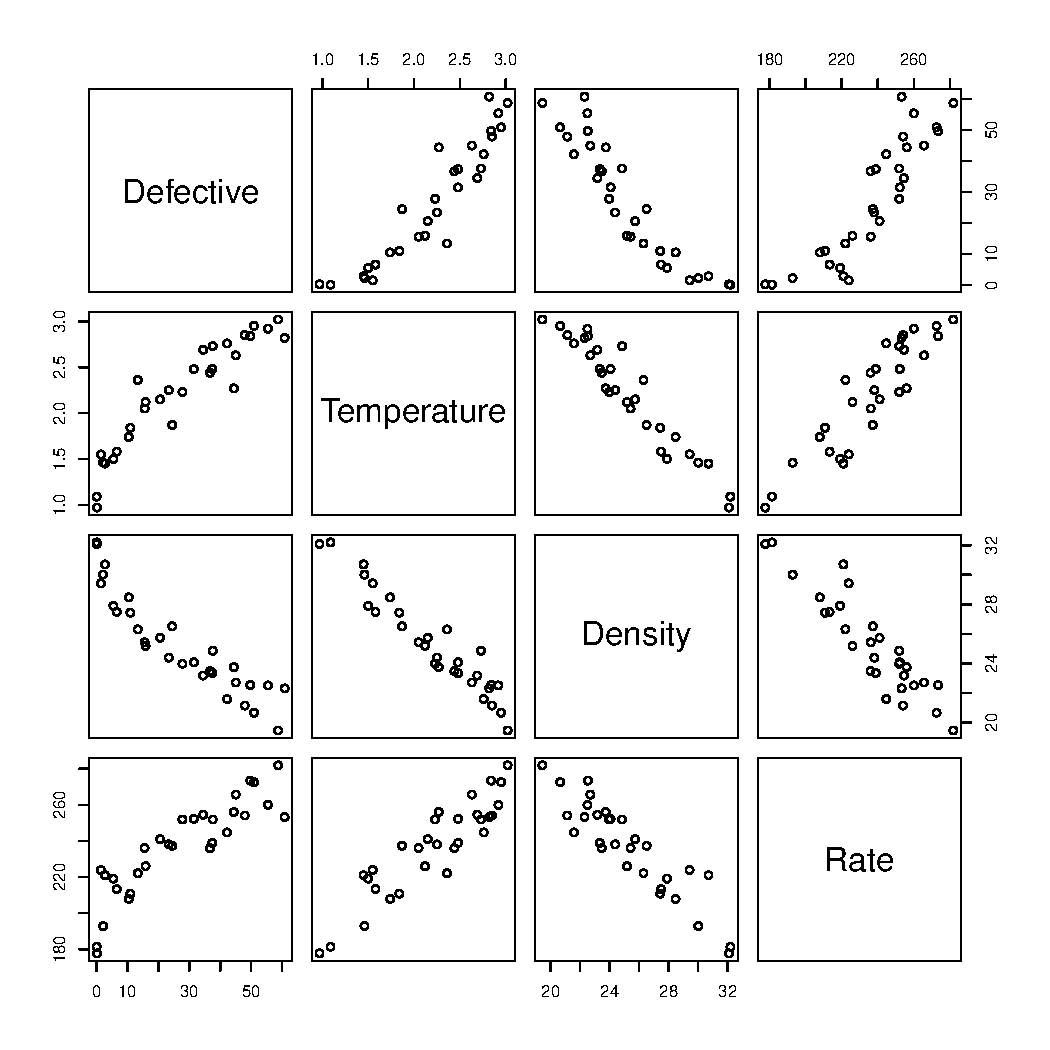
\includegraphics[scale=0.4]{figure/defects_pairs1.pdf}
\end{figure}
\end{frame}

\begin{frame}[fragile]
The scatterplot matrix and residual versus fitted plot show nonlinearity in the data that is not accounted for by the linear regression model.
\small
\begin{verbatim}
> lm1 <- lm(Defective ~ Temperature + Density + Rate, data=defects)
> par(mfrow=c(1,2), mar=c(4.5, 4.5, 2, 2))
> plot(lm1, 1:2)
\end{verbatim}
\begin{figure}
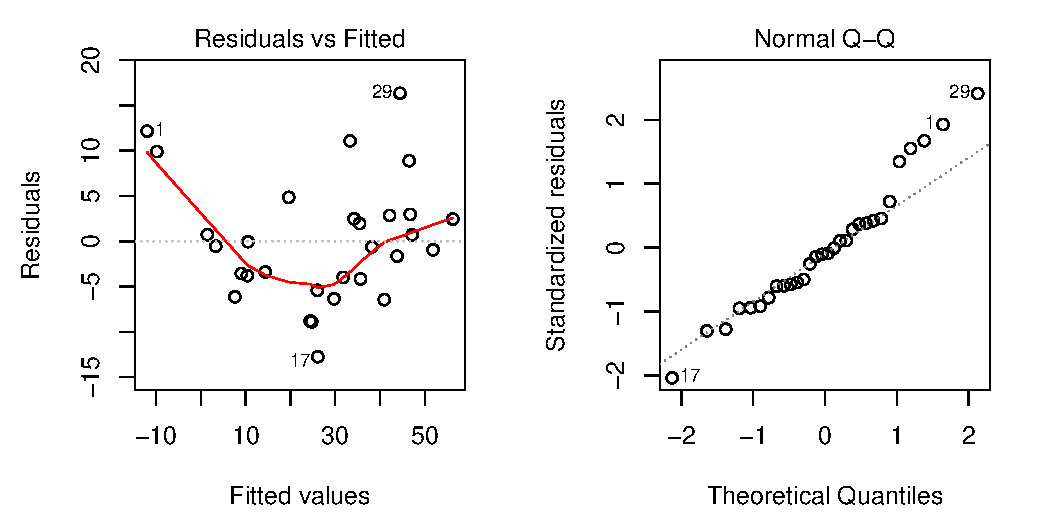
\includegraphics[scale=0.5]{figure/defects_resid1.pdf}
\end{figure}
\end{frame}

\begin{frame}[fragile]
\scriptsize
\begin{verbatim}
> par(mfrow=c(1,3), mar=c(4.5, 4.5, 2, 2))
> plot(defects$Temperature, rstandard(lm1), 
       xlab="Temperature", ylab="Standardized Residuals")
> plot(defects$Density, rstandard(lm1), 
       xlab="Density", ylab="Standardized Residuals")
> plot(defects$Rate, rstandard(lm1), 
       xlab="Rate", ylab="Standardized Residuals")
\end{verbatim}
\begin{figure}
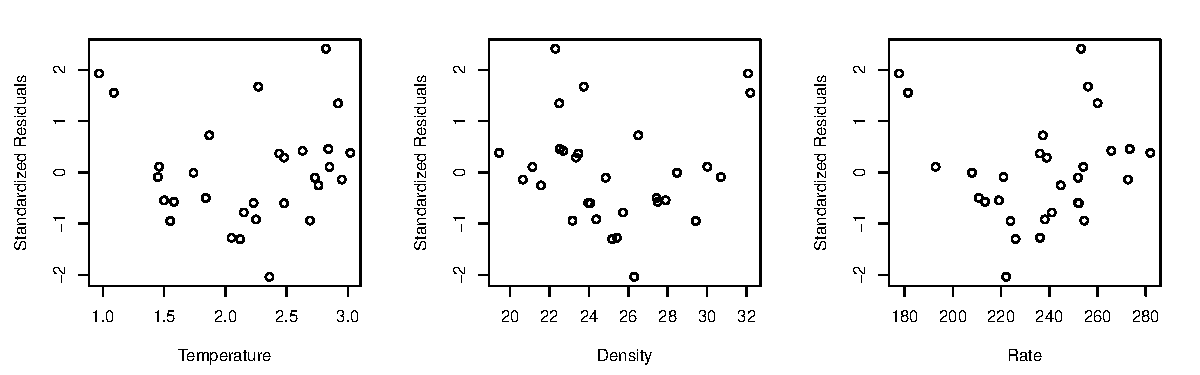
\includegraphics[scale=0.55]{figure/defects_resid_x1.pdf}
\end{figure}
\end{frame}



\begin{frame}[fragile]
\small
\begin{verbatim}
> library(MASS)
> library(car)
> boxcox(lm1, lambda=seq(0.3, 0.65, by=0.05))
> summary(powerTransform(lm1))
bcPower Transformation to Normality 
   Est Power Rounded Pwr Wald Lwr Bnd Wald Upr Bnd
Y1    0.4519         0.5       0.3253       0.5785
\end{verbatim}
\begin{figure}
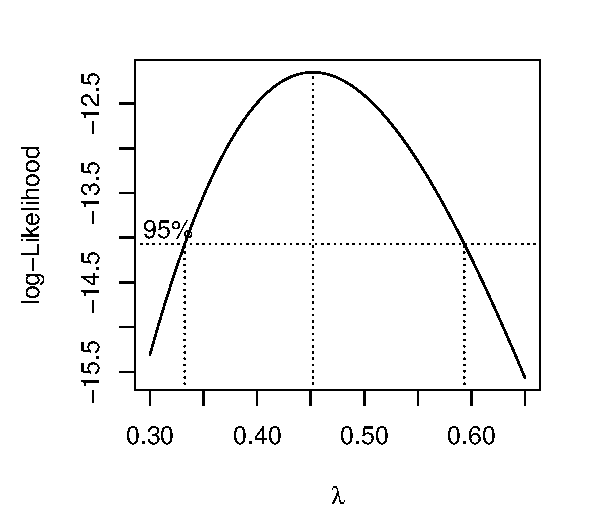
\includegraphics[scale=0.55]{figure/defects_boxcox.pdf}
\end{figure}
\end{frame}

\begin{frame}
\begin{itemize}
\item Using the Box-Cox procedure, the estimated value of the parameter is $\hat{\lambda} = 0.45$.
\vspace{5pt}
\item The 95\% confidence interval for $\lambda$ is between 0.33 and 0.58.  
\vspace{5pt}
\item For interpretability, we will round and use $Y^{0.5}$, the square root transformation.
\vspace{5pt}
\item Thus, the regression model with the transformed response is
\begin{align*}
\sqrt{Y} = \beta_0 + \beta_1 x_1 + \beta_2 x_2 + \beta_3 x_3 + e
\end{align*}
\end{itemize}
\end{frame}

\begin{frame}[fragile]
The regression equation is given by:
$$\widehat{\sqrt{Y}} = 5.593 + 1.565 x_1 - 0.292 x_2 + 0.013 x_3$$
\small
\begin{verbatim}
> lm2 <- lm(sqrt(Defective) ~ Temperature + Density + Rate, 
            data=defects)
> summary(lm2)
Coefficients:
            Estimate Std. Error t value Pr(>|t|)  
(Intercept)  5.59297    5.26401   1.062   0.2978  
Temperature  1.56516    0.66226   2.363   0.0259 *
Density     -0.29166    0.11954  -2.440   0.0218 *
Rate         0.01290    0.01043   1.237   0.2273  
---
Signif. codes:  0 ‘***’ 0.001 ‘**’ 0.01 ‘*’ 0.05 ‘.’ 0.1 ‘ ’ 1

Residual standard error: 0.5677 on 26 degrees of freedom
Multiple R-squared:  0.943,	Adjusted R-squared:  0.9365 
F-statistic: 143.5 on 3 and 26 DF,  p-value: 2.713e-16
\end{verbatim}

\end{frame}

\begin{frame}[fragile]
After making the transformation, the plots of the residuals versus fitted values, and residuals versus each predictor, are much improved.  The points appear to be randomly scattered in each plot, and show no obvious patterns or nonconstant variance.  Thus, the transformed model appears to fit the data reasonably well.  
\small
\begin{verbatim}
> par(mfrow=c(1,2), mar=c(4.5, 4.5, 2, 2))
> plot(lm2, 1:2)
\end{verbatim}
\begin{figure}
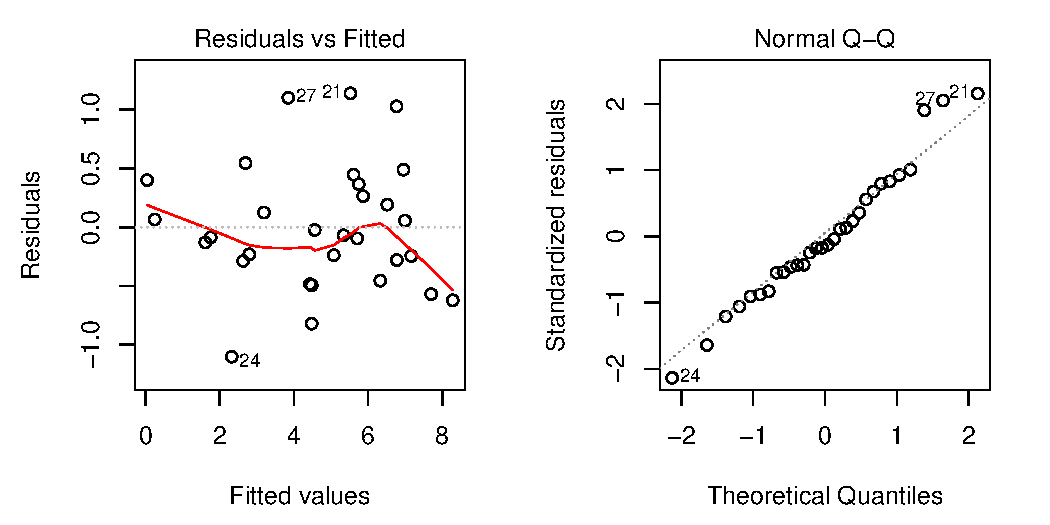
\includegraphics[scale=0.5]{figure/defects_resid2.pdf}
\end{figure}
\end{frame}

\begin{frame}[fragile]
\scriptsize
\begin{verbatim}
> par(mfrow=c(1,3), mar=c(4.5, 4.5, 2, 2))
> plot(defects$Temperature, rstandard(lm2), 
       xlab="Temperature", ylab="Standardized Residuals")
> plot(defects$Density, rstandard(lm2), 
       xlab="Density", ylab="Standardized Residuals")
> plot(defects$Rate, rstandard(lm2), 
       xlab="Rate", ylab="Standardized Residuals")
\end{verbatim}
\begin{figure}
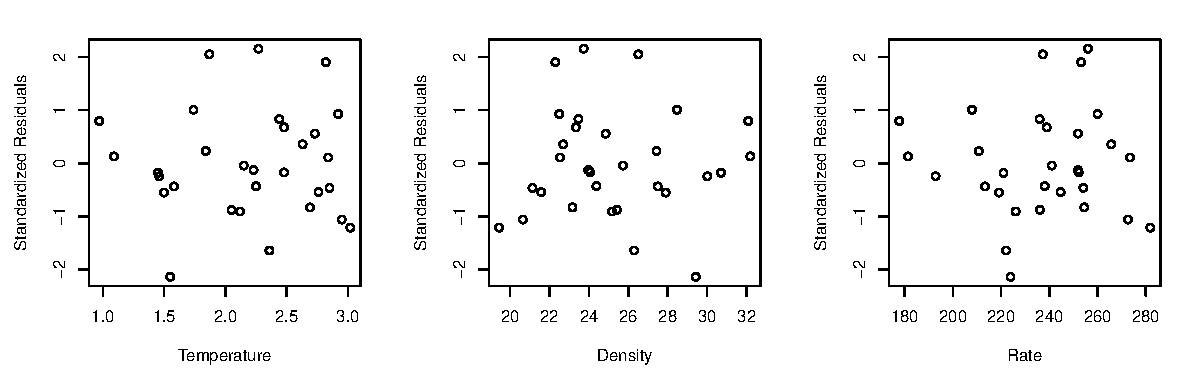
\includegraphics[scale=0.55]{figure/defects_resid_x2.pdf}
\end{figure}
\end{frame}

\begin{frame}
Another useful diagnostic is a plot of the observed versus fitted values.  Ideally, we should see a straight line relationship (around the 1-1 line).  In the plots below, we see that before transforming the response, the relationship is curved; while after transforming the response, the relationship is straight.  The loess curve is shown in red.
\begin{figure}
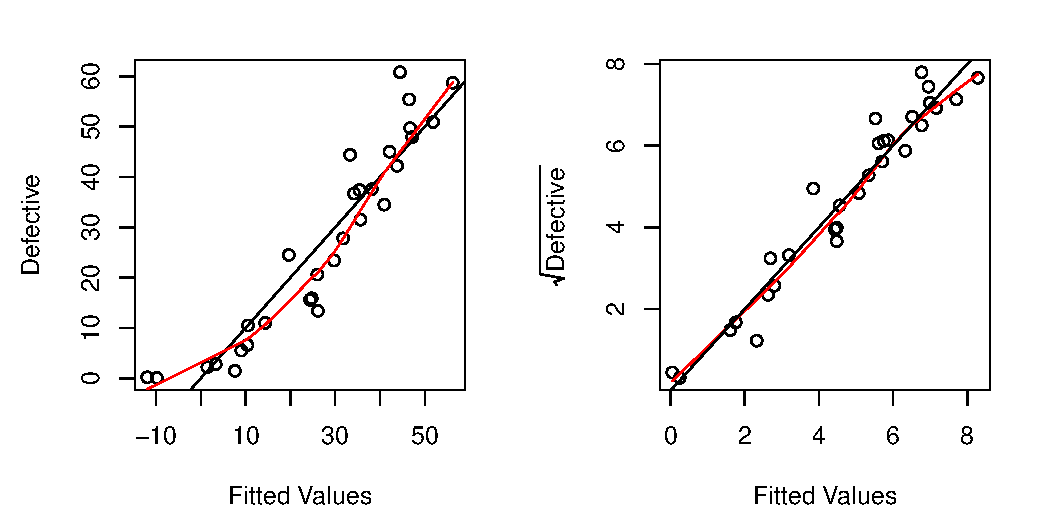
\includegraphics[scale=0.55]{figure/defects_obs_pred.pdf}
\end{figure}
\end{frame}

\begin{frame}[fragile]
The code used to generate the last plot:
\small
\begin{verbatim}
> par(mfrow=c(1,2), mar=c(4.5, 4.5, 2, 2))
> plot(predict(lm1), defects$Defective, 
       xlab = "Fitted Values", ylab = "Defective")
> abline(0,1)
> lines(lowess(predict(lm1), defects$Defective), col='red')

> plot(predict(lm2), sqrt(defects$Defective), 
       xlab = "Fitted Values", ylab = expression(sqrt(Defective)))
> lines(lowess(predict(lm2), sqrt(defects$Defective)), col='red')
> abline(0,1)
\end{verbatim}
\end{frame}

\begin{frame}{Transforming the Predictors}
\begin{itemize}
\item Inspection of the scatterplot matrix can sometimes indicate whether or not to log transform a predictor.  
\vspace{5pt}
\item Recall, that the log transformation is useful when the data are skewed and/or range over several orders of magnitude.
\vspace{5pt}
\item Other types of transformations, such as the square root, can also be considered for the predictors.  
\vspace{5pt}
\item Once transformations have been chosen for the predictors, the Box-Cox method can be used to estimate a transformation for the response.
\end{itemize}
\end{frame}

\begin{frame}{Summary and Remarks}
\begin{itemize}
\item The Box-Cox method is a useful technique for transforming the response variable.
\vspace{5pt}
\item Box-Cox transformations can help linearize the relationship between the response and the predictors, and also overcome problems due to nonconstant variability.
\vspace{5pt}
\item Scatterplot matrices and residual plots should also be used when determining transformations.  Do not just rely on automated procedures, also make sure to look at your data.
\end{itemize}
\end{frame}

\begin{frame}{Summary and Remarks}
\begin{itemize}
\item We can round $\lambda$ to the nearest interpretable value.  For example, if $\hat{\lambda} = 0.45$  then we can use  $\sqrt{y}$ as the transformation.  The confidence interval for $\lambda$ can be used as an aid to determine the rounding.
\vspace{5pt}
\item Transformations can make the model more difficult to interpret.  So if $\hat{\lambda} \approx 1$ and the confidence interval for $\lambda$ contains 1, a transformation is probably not necessary.
\vspace{5pt}
\item For $\lambda > 0$, we can just use $y^{\lambda}$ as the response transformation (no need to use the formal scaling $(y^{\lambda}-1)/\lambda$).
\vspace{5pt}
\item If some $y_i \leq 0$ we can add a small constant to make all the $y$ data positive.
\vspace{5pt}
\item There is usually little justification for making extreme transformations such as $\hat{\lambda} = 5$.
\end{itemize}
\end{frame}

\begin{frame}[fragile]{Your turn}
Consider the New York City restaurant price data:
\begin{verbatim}
nyc <- read.csv("https://ericwfox.github.io/data/nyc.csv")
lm2 <- lm(Price ~ Food + Decor + East, data=nyc)
\end{verbatim}
Use the \texttt{boxcox()} function to plot the log-likelihood and find a confidence interval for $\lambda$.  Based on these results, does it seem necessary to transform the response?
\end{frame}



\end{document}
